\subsubsection{GeneRec}

\paragraph{Introduction - version 1} 
The algorithm GeneRec (Generic Recirculation), developed by O’Reilly \citet{o1996bio} based on back-propagation, is argued to be a more biologically plausible supervised learning algorithm: learning happens through synaptic weight modifications using only local information available in synapses. In summary, GeneRec is a generalized version of the recirculation algorithm \citet{hinton1988learning}, which overcomes the limitations of the earlier algorithm (ex.: back-propagation) by using a generic recurrent network with sigmoidal units that can learn arbitrary input and output mappings. GeneRec employs two phases: \emph{minus} and \emph{plus} \citet{da2011advances}. 

\paragraph{Introduction - version 2} 
Learning is done by the Generalized Recirculation
(GeneRec) algorithm, which is argued to be a more bio-
logically plausible form of learning, developed by O’Reilly
[9]. One motivation of the development of GeneRec was
the treatment of typical problems encountered in the
backpropagation algorithm when working with bidirec-
tional networks. There is propagation of two signals in
GeneRec: the expectation of the network (called \emph{minus}
phase) and the training signal (also called \emph{plus} phase).
\citet{schneider2009application} 

\begin{table}
  \centering
  \caption{Equilibrium network variables in GeneRec model \citet{farkas2013bal}.}
  \label{tab:gr-states}
  \begin{tabular}{|cccc|}
    \hline
    Layer & Phase & Net Input & Activation\\
    \hline
    Input (s)    & $-$ & - & $s_i$ = stimulus input\\
    \hline
    Hidden (h)   & $-$ & \hspace{0.3cm}$\eta^{-}_j = \sum_i w_{ij}s_i + \sum_k w_{kj}o^{-}_k$\hspace{0.3cm} &
    $h^{-}_j = \sigma(\eta^{-}_j)$\hspace{0.3cm}\\
          &  +  & $\eta^{+}_j = \sum_{i}w_{ij}s_i + \sum_k w_{kj}o^{+}_k$ & $h^{+}_{j} = \sigma(\eta^{+}_j)$ \\
    \hline
    Output (o) & $-$ & $\eta^{-}_k = \sum_j w_{jk}h_j$ & $o^{-}_k = \sigma(\eta^{-}_k)$\\
           &  +  & - & $o^{+}_k$ = target output \\
    \hline
  \end{tabular}
\end{table}

The basic weight update rule in GeneRec is:
\begin{equation}
  \Delta w_{pq} = \lambda \ a^{-}_p(a^{+}_q - a^{-}_q)
\label{eq:generec}
\end{equation}
where $a^{-}_p$ denotes the presynaptic and $a^{-}_q$ denotes the postsynaptic unit activation in minus phase, $a^{+}_p$ is the presynaptic activation from plus phase (in output-to-hidden direction) and $\lambda$ denotes the learning rate. The learning rule given in Eq.~\ref{eq:generec} is applied to both input-hidden and hidden-output weights.  Due to the lack of space, the reader is left to consult the original paper \citet{o1996bio} regarding the underlying math behind the derivation of the GeneRec learning rule.

\paragraph{Minus phase.} When units xi are presented to the input layer A, there is the propagation of this stimulus to the hidden layer B (bottom-up propagation) (figure 1). At the same time, the previous output ok propagates from the output layer C to the hidden layer B (top- down propagation) (figure 2). Then the hidden activation \emph{minus} - minus phase - ($h^-$ ) is generated (sum of bottom-up and top-down propagations). The activation function $\sigma$ is sigmoid. Equation 1 shows the hidden activation calculus for one hidden unit j. wij are the synaptic weights from the input layer to the hidden layer and wjk are the synaptic weights from the hidden layer to the output layer (which are the same as the weights from the output layer to the hidden layer, because reciprocal weights are symmetric in GeneRec, that is, wjk = wkj \citet{o1996bio}). ok(t-1) is the previous output (output on time t - 1) \citet{orru2008sabio}.

$$h_j^- = \sigma \left(\sum_{i=0}^A w_{ij} \cdot x_i + \sum_{k=1}^C w_{jk} \cdot o_k(t-1)\right)$$

Finally, the real output ok(t) is generated through the propagation of the \emph{minus} layer activation to the output layer (figure 3), shown for one output unit k by equation 2 \citet{o1996bio}. Notice that the architecture employed is bi-directional. Recall that ok (t) (the current output on time t) is used in order to differentiate it from ok (t - 1) (the previous output on time t - 1).

\begin{center} 
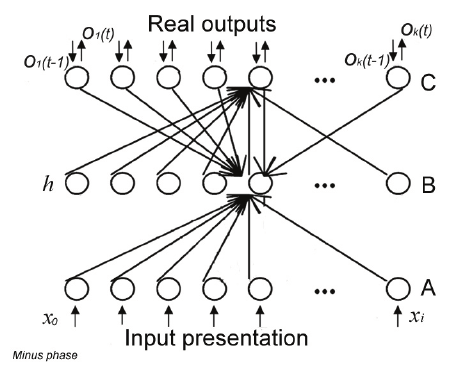
\includegraphics{img/generec_minus_phase.png} \citet{orru2008sabio} 
\end{center} 

\paragraph{Plus phase.} Units xi are presented again to the input layer A; there is the propagation of this stimulus to the hidden layer B (bottom-up propagation) (figure 4). At the same time, the desired output yk propagates from the output layer C to the hidden layer B (top- down propagation) (figure 5). Then the hidden activation + \emph{plus} - plus phase - (hj) is generated, summin bottom-up and top-down propagations (equation 3) \citet{o1996bio}, \citet{orru2008sabio}.

$$h_j^+ = \sigma\left( \sum_{i=0}^A w_{ij} \cdot x_i + \sum_{k=1}^C w_{jk} y_k \right)$$

\begin{center} 
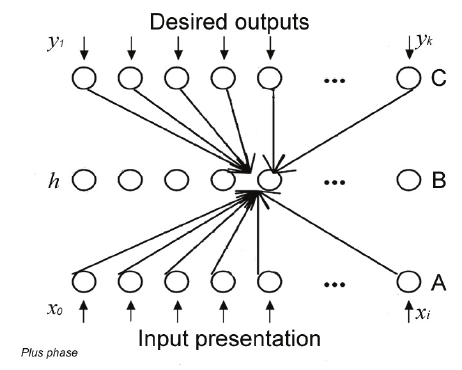
\includegraphics{img/generec_plus_phase.png} \citet{orru2008sabio} 
\end{center} 

In order to make learning possible, synaptic weights $w$ are updated, based on h-, j  $h^+_j$, $o_k$ , $y_k$, $x_i$, and the learning rate $\eta$ (equations 4 and 5).

%TODO equation labels with intext references 
$$\Delta w_{jk} = \eta(y_k - o_k(t)) h^-_j $$

$$\Delta w_{ij} = \eta(h^+_j - h^-_j) x_i$$

Finally, O’Reilly \citet{o1998six} suggests, unlike backpropagation, that the teaching signal is just another state of “experience” in the network, that is, in GeneRec algorithm the teaching signal is exactly the “top-down” activation in the plus-phase.


%TODO reformulate 
It was recently shown that backpropagation can be implemented in a more biologically plausible fashion using bidirectional activation propagation in an interactive network using the GeneRec algorithm \citet{o1996bio}, which is a generalization of the recirculation algorithm \citet{hinton1988learning}. In GeneRec, error information is propagated as two separate terms via standard activation propagation mechanisms in interactive networks, and the difference between these terms (which is the error signal) can be plausibly computed using the synaptic modification mechanisms underlying long term potentiation and depression (LTP/LTD). Versions of the GeneRec algorithm are equivalent to the other known ways of implementing powerful error-driven learning using interactive activation propagation instead of direct error propagation (e.g., the deterministic Boltzmann machine \citet{hinton1989deterministic} and Contrastive Hebbian Learning \citet{movellan1990contrastive}). Thus, several different approaches converge on the idea that the way to perform error-driven learning in a more biologically plausible manner is to use interactive networks, where error signals are communicated via top-down activation propagation \citet{o2001generalization}.

Copy from \citet{da2011advances} 


%TODO try out the following rules: 
Hebbian learning is performed using a Conditional Principal Components Analysis (CPCA) algorithm with a correction factor for sparse expected activity levels [3]. The error-driven learning is achieved with GeneRec; the output is computed in two phases – an expectation phase where the network's actual output is produced and an outcome phase where the target output is experienced – as a difference of a pre- and postsynaptic activation product across these two phases. Hebbian weights are adjusted according to the following formula.

equation image	(2)
while error-driven learning uses the following equation.

equation image	(3)
where xi is the input of neuron i, yj is the output of neuron j, and wij is the connection weight between neurons i and j. The “+” and “– superscripts refer to plus and minus phases of the GeneRec algorithm \citet{nawrocki2012monitoring}.

Some improvements \citet{da2008biological}. 

To assess the effect of interactivity, two different networks were compared on the combinatorial generalization task, a standard feedforward backpropagation network, and an interactive GeneRec network using the symmetric, midpoint variation learning rule which is equivalent to contrastive Hebbian learning (CHL) or a deterministic Boltzmann machine (DBM) \citet{o1996bio}, \citet{o2001generalization}. 
 
\footnote{TODO: How to cope with biases (which are not symmetric)? We haven't found how GeneRec uses the Bias neuron.} 
